\section*{Aufgabe 1}

\subsection*{a)}
\begin{tabular}{l  l  c}
$\forall w \in \Sigma^{*}$ wo gilt $ w \in L(N) $ & $\Leftrightarrow \widehat{\delta} (q_0 , w) \subseteq F$ & (Def $NEA_{BUG}$) \\
& $\Leftrightarrow \widehat{\delta} (q_0 , w) \cap F \neq \emptyset$ & (Def Akzeptanz) \\
& $\Leftrightarrow \widehat{\delta} (q_0 , w) \cap \emptyset \neq \emptyset$ & ( $F= \emptyset $) \\
& $\Leftrightarrow \emptyset \neq \emptyset$ & ( $Set \cap \emptyset = \emptyset $) \\
 Widerspruch  & $\Rightarrow w \not \in L(N)$ $ \forall w \in \Sigma^{*} $ \\
 & $\Rightarrow  L(N) = \emptyset$ &
\end{tabular}
\subsection*{b)}
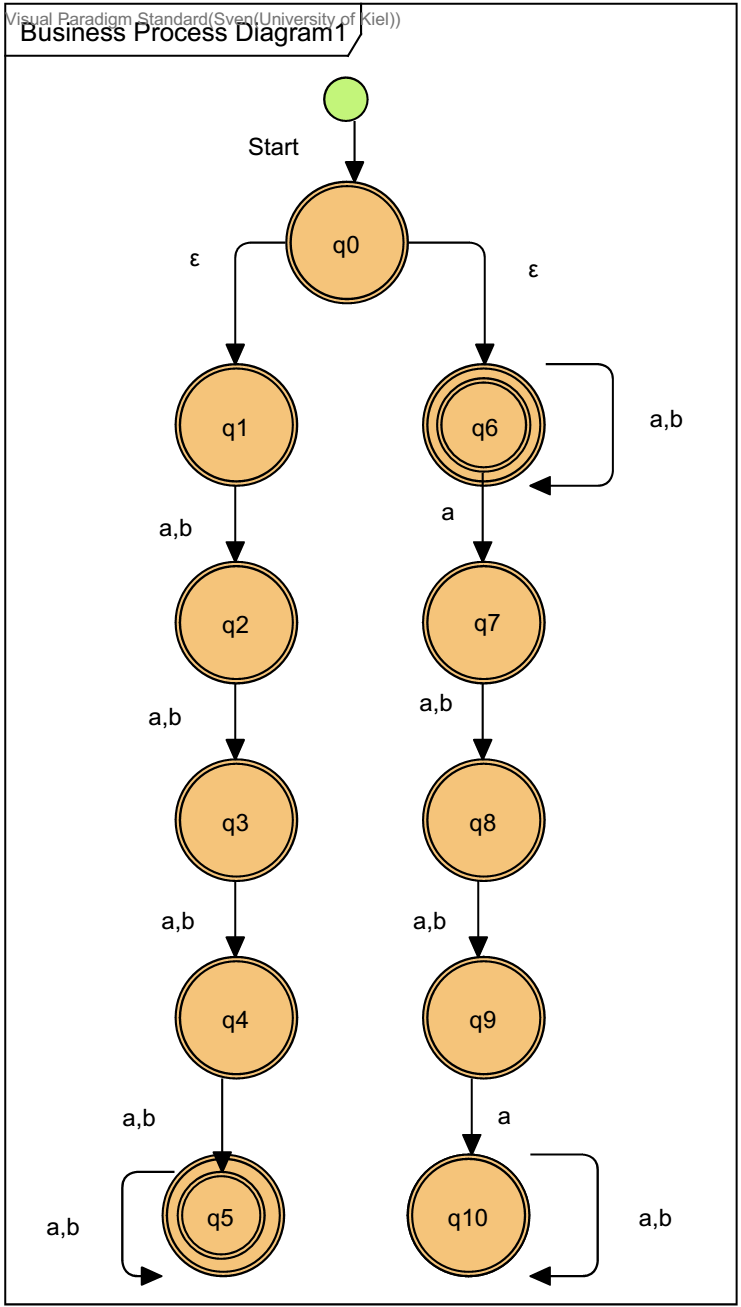
\includegraphics[scale=0.4]{part/TGIS09A01b.png}
\subsection*{c)}
Sei M $DEA$  mit $M=(P (Q), \Sigma , \delta^{*} , \{ q_0\}, P(P (F)))$ Deterministischer Automat zu $N=(Q, \Sigma , \delta , q_0,F) \in NEA_{BUG}$ und:\\
 1) $P(Q) =$ Potenzmenge von $Q $\\
 2) $\Sigma$ wie in $N$\\
 3) $ \delta^{*}(r,a) = \bigcup_{s \in r} \delta(s,a)$\\
 4) ${q_0} $ mit $q_0 $aus N\\
 5) $P (Q) $ Potenzmenge der Potenzmenge von $F$\\
 \\
Beweis:\\
\begin{tabular}{l  l  c}
$w \in L(M)$ & $\Leftrightarrow \widehat{\delta^*} (\{q_0\} , w) \in P(P(F))$ & (Def $M$) \\
& $\Leftrightarrow \widehat{\delta} (q_0 , w) \in  P(F)) $ & (Def $ \delta^* $)\\
& $\Leftrightarrow \widehat{\delta} (q_0 , w) \subseteq  F $ & (Def $ P(F) $)\\
& $ \Leftrightarrow w \in L(N) $ & (Def $ N $)\\
\end{tabular} 
 
\subsection*{d)} 
 Nicht regulär möglich dass ein Reg Audruck verbunden ist nicht von einem $ NEA_{BUG}$ erkannt werden kann
